% Options for packages loaded elsewhere
\PassOptionsToPackage{unicode}{hyperref}
\PassOptionsToPackage{hyphens}{url}
%
\documentclass[
]{book}
\usepackage{amsmath,amssymb}
\usepackage{lmodern}
\usepackage{iftex}
\ifPDFTeX
  \usepackage[T1]{fontenc}
  \usepackage[utf8]{inputenc}
  \usepackage{textcomp} % provide euro and other symbols
\else % if luatex or xetex
  \usepackage{unicode-math}
  \defaultfontfeatures{Scale=MatchLowercase}
  \defaultfontfeatures[\rmfamily]{Ligatures=TeX,Scale=1}
\fi
% Use upquote if available, for straight quotes in verbatim environments
\IfFileExists{upquote.sty}{\usepackage{upquote}}{}
\IfFileExists{microtype.sty}{% use microtype if available
  \usepackage[]{microtype}
  \UseMicrotypeSet[protrusion]{basicmath} % disable protrusion for tt fonts
}{}
\makeatletter
\@ifundefined{KOMAClassName}{% if non-KOMA class
  \IfFileExists{parskip.sty}{%
    \usepackage{parskip}
  }{% else
    \setlength{\parindent}{0pt}
    \setlength{\parskip}{6pt plus 2pt minus 1pt}}
}{% if KOMA class
  \KOMAoptions{parskip=half}}
\makeatother
\usepackage{xcolor}
\IfFileExists{xurl.sty}{\usepackage{xurl}}{} % add URL line breaks if available
\IfFileExists{bookmark.sty}{\usepackage{bookmark}}{\usepackage{hyperref}}
\hypersetup{
  pdftitle={VECTORES AUTOREGRESIVOS (VAR)},
  pdfauthor={Luis Ortiz-Cevallos},
  hidelinks,
  pdfcreator={LaTeX via pandoc}}
\urlstyle{same} % disable monospaced font for URLs
\usepackage{color}
\usepackage{fancyvrb}
\newcommand{\VerbBar}{|}
\newcommand{\VERB}{\Verb[commandchars=\\\{\}]}
\DefineVerbatimEnvironment{Highlighting}{Verbatim}{commandchars=\\\{\}}
% Add ',fontsize=\small' for more characters per line
\usepackage{framed}
\definecolor{shadecolor}{RGB}{248,248,248}
\newenvironment{Shaded}{\begin{snugshade}}{\end{snugshade}}
\newcommand{\AlertTok}[1]{\textcolor[rgb]{0.94,0.16,0.16}{#1}}
\newcommand{\AnnotationTok}[1]{\textcolor[rgb]{0.56,0.35,0.01}{\textbf{\textit{#1}}}}
\newcommand{\AttributeTok}[1]{\textcolor[rgb]{0.77,0.63,0.00}{#1}}
\newcommand{\BaseNTok}[1]{\textcolor[rgb]{0.00,0.00,0.81}{#1}}
\newcommand{\BuiltInTok}[1]{#1}
\newcommand{\CharTok}[1]{\textcolor[rgb]{0.31,0.60,0.02}{#1}}
\newcommand{\CommentTok}[1]{\textcolor[rgb]{0.56,0.35,0.01}{\textit{#1}}}
\newcommand{\CommentVarTok}[1]{\textcolor[rgb]{0.56,0.35,0.01}{\textbf{\textit{#1}}}}
\newcommand{\ConstantTok}[1]{\textcolor[rgb]{0.00,0.00,0.00}{#1}}
\newcommand{\ControlFlowTok}[1]{\textcolor[rgb]{0.13,0.29,0.53}{\textbf{#1}}}
\newcommand{\DataTypeTok}[1]{\textcolor[rgb]{0.13,0.29,0.53}{#1}}
\newcommand{\DecValTok}[1]{\textcolor[rgb]{0.00,0.00,0.81}{#1}}
\newcommand{\DocumentationTok}[1]{\textcolor[rgb]{0.56,0.35,0.01}{\textbf{\textit{#1}}}}
\newcommand{\ErrorTok}[1]{\textcolor[rgb]{0.64,0.00,0.00}{\textbf{#1}}}
\newcommand{\ExtensionTok}[1]{#1}
\newcommand{\FloatTok}[1]{\textcolor[rgb]{0.00,0.00,0.81}{#1}}
\newcommand{\FunctionTok}[1]{\textcolor[rgb]{0.00,0.00,0.00}{#1}}
\newcommand{\ImportTok}[1]{#1}
\newcommand{\InformationTok}[1]{\textcolor[rgb]{0.56,0.35,0.01}{\textbf{\textit{#1}}}}
\newcommand{\KeywordTok}[1]{\textcolor[rgb]{0.13,0.29,0.53}{\textbf{#1}}}
\newcommand{\NormalTok}[1]{#1}
\newcommand{\OperatorTok}[1]{\textcolor[rgb]{0.81,0.36,0.00}{\textbf{#1}}}
\newcommand{\OtherTok}[1]{\textcolor[rgb]{0.56,0.35,0.01}{#1}}
\newcommand{\PreprocessorTok}[1]{\textcolor[rgb]{0.56,0.35,0.01}{\textit{#1}}}
\newcommand{\RegionMarkerTok}[1]{#1}
\newcommand{\SpecialCharTok}[1]{\textcolor[rgb]{0.00,0.00,0.00}{#1}}
\newcommand{\SpecialStringTok}[1]{\textcolor[rgb]{0.31,0.60,0.02}{#1}}
\newcommand{\StringTok}[1]{\textcolor[rgb]{0.31,0.60,0.02}{#1}}
\newcommand{\VariableTok}[1]{\textcolor[rgb]{0.00,0.00,0.00}{#1}}
\newcommand{\VerbatimStringTok}[1]{\textcolor[rgb]{0.31,0.60,0.02}{#1}}
\newcommand{\WarningTok}[1]{\textcolor[rgb]{0.56,0.35,0.01}{\textbf{\textit{#1}}}}
\usepackage{longtable,booktabs,array}
\usepackage{calc} % for calculating minipage widths
% Correct order of tables after \paragraph or \subparagraph
\usepackage{etoolbox}
\makeatletter
\patchcmd\longtable{\par}{\if@noskipsec\mbox{}\fi\par}{}{}
\makeatother
% Allow footnotes in longtable head/foot
\IfFileExists{footnotehyper.sty}{\usepackage{footnotehyper}}{\usepackage{footnote}}
\makesavenoteenv{longtable}
\usepackage{graphicx}
\makeatletter
\def\maxwidth{\ifdim\Gin@nat@width>\linewidth\linewidth\else\Gin@nat@width\fi}
\def\maxheight{\ifdim\Gin@nat@height>\textheight\textheight\else\Gin@nat@height\fi}
\makeatother
% Scale images if necessary, so that they will not overflow the page
% margins by default, and it is still possible to overwrite the defaults
% using explicit options in \includegraphics[width, height, ...]{}
\setkeys{Gin}{width=\maxwidth,height=\maxheight,keepaspectratio}
% Set default figure placement to htbp
\makeatletter
\def\fps@figure{htbp}
\makeatother
\setlength{\emergencystretch}{3em} % prevent overfull lines
\providecommand{\tightlist}{%
  \setlength{\itemsep}{0pt}\setlength{\parskip}{0pt}}
\setcounter{secnumdepth}{5}
\ifLuaTeX
  \usepackage{selnolig}  % disable illegal ligatures
\fi
\usepackage[]{natbib}
\bibliographystyle{apalike}

\title{VECTORES AUTOREGRESIVOS (VAR)}
\author{\href{https://ortiz-cevallos.github.io/MYSELF/}{Luis Ortiz-Cevallos}}
\date{2022-03-07}

\begin{document}
\maketitle

{
\setcounter{tocdepth}{1}
\tableofcontents
}
\hypertarget{introducciuxf3n}{%
\chapter{INTRODUCCIÓN}\label{introducciuxf3n}}

\hypertarget{paquete-en-r}{%
\section{Paquete en R}\label{paquete-en-r}}

En esta nota para la obtención de un Vector Autorregresivo Estructural (SVAR) se utilizará el paquete en R \emph{SVARS} elaborado por \citet{SVAR21}. A continuación se muestra la carga de este paquete junto a otros que serán de utilidad cuando se analicen los resultados.

\begin{Shaded}
\begin{Highlighting}[]
\CommentTok{\#install.packages("svars")}
\FunctionTok{library}\NormalTok{(}\StringTok{"svars"}\NormalTok{)}
\FunctionTok{library}\NormalTok{(}\StringTok{"ggplot2"}\NormalTok{)}
\end{Highlighting}
\end{Shaded}

Enseguida se cargará una base de datos en frecuencia trimestral que contiene la brecha producto, la inflación de trimestre a trimestre del deflactor del PIB y una tasa de interés nominal del fondo federal.

\begin{Shaded}
\begin{Highlighting}[]
\FunctionTok{data}\NormalTok{(}\StringTok{"USA"}\NormalTok{)}
\NormalTok{usa}\OtherTok{\textless{}{-}}\FunctionTok{as.zoo}\NormalTok{(USA)}
\end{Highlighting}
\end{Shaded}

A continuación se replicará los resultados obtenidos por \citet{Herwartz2016}, específicamente se estimaran los shocks estructurales a través de la metodología de cambios en volatilidades. Ello se logra a través de la función \emph{id.cv()} dentro del cual hay que indicarle la fecha a partir de la cual se dio ese cambio estructural.

\citet{Herwartz2016} argumentan que el punto de quiebra se dio en el tercer trimestre de 1979 donde aconteció un cambio en la política de la Reserva Federal que redujo la volatilidad de las variables macroeconómicas (ver \citet{Stock2003})

Lo anterior es posible visualizarlo.
Un primer paso es visualizar cada una de las series.

\begin{Shaded}
\begin{Highlighting}[]
\FunctionTok{autoplot}\NormalTok{(usa, }\AttributeTok{facets =}\NormalTok{ T) }\SpecialCharTok{+} \FunctionTok{theme\_bw}\NormalTok{() }\SpecialCharTok{+} \FunctionTok{ylab}\NormalTok{(}\StringTok{\textquotesingle{}Evolución de series de USA\textquotesingle{}}\NormalTok{)}
\end{Highlighting}
\end{Shaded}

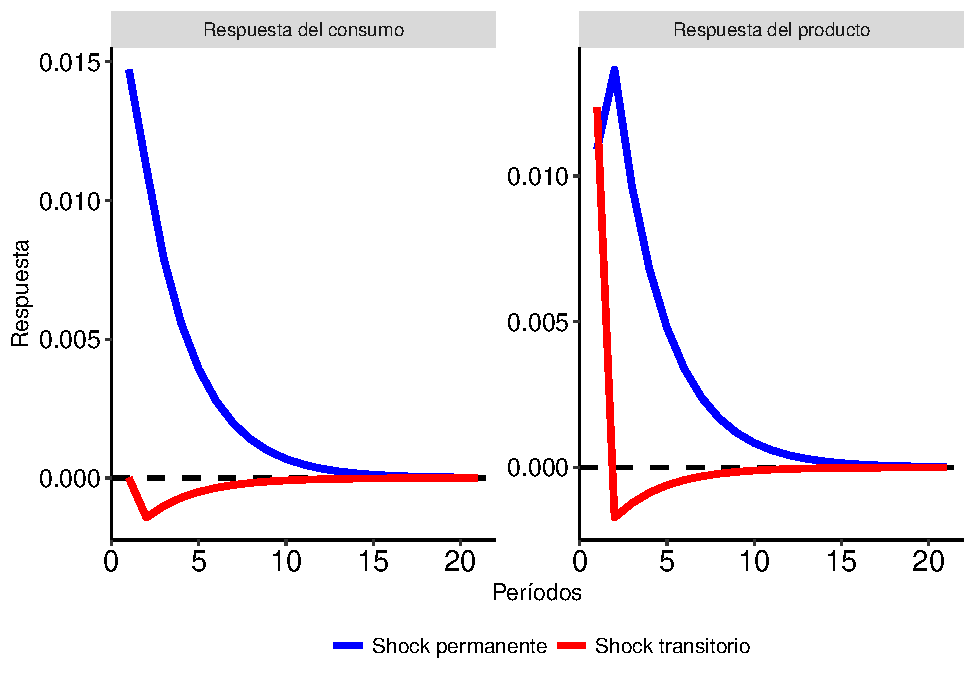
\includegraphics{01-conceptos_files/figure-latex/unnamed-chunk-3-1.pdf}

Seguidamente se estimara la forma reducida de un VAR, aplicaremos una especificación que incluya intercepto y hasta seis rezagos (p=6)

\begin{Shaded}
\begin{Highlighting}[]
\NormalTok{plain.var }\OtherTok{\textless{}{-}}\NormalTok{ vars}\SpecialCharTok{::}\FunctionTok{VAR}\NormalTok{(USA, }\AttributeTok{p =} \DecValTok{6}\NormalTok{, }\AttributeTok{type =} \StringTok{\textquotesingle{}const\textquotesingle{}}\NormalTok{)}
\end{Highlighting}
\end{Shaded}

Con base en el objeto VAR podemos estimar su forma estructural con la función \emph{id.cv()} la cual introduce el \emph{cambio en la varianza} que se observa en las series, sin embargo la aplicación de esta función requiere específicar el argumento \emph{SB} en formato \emph{ts}:

\begin{Shaded}
\begin{Highlighting}[]
\NormalTok{usa.cv }\OtherTok{\textless{}{-}} \FunctionTok{id.cv}\NormalTok{(plain.var, }\AttributeTok{SB =} \FunctionTok{c}\NormalTok{(}\DecValTok{1979}\NormalTok{, }\DecValTok{3}\NormalTok{))}
\FunctionTok{summary}\NormalTok{(usa.cv)}
\end{Highlighting}
\end{Shaded}

\begin{verbatim}
## 
## Identification Results
## ---------------------- 
## 
## Method: Changes in Volatility
## Sample size: 169
## Log-Likelihood: -564.2994
## AIC: 1268.599
## Structural Break: At Observation Number 59 during 1979 Q3
## Number of GLS estimations: 22
## Number of Restrictions: 0
## 
## Estimated unconditional Heteroscedasticity Matrix (Lambda):
##         [,1]     [,2]     [,3]
## x  0.3925906 0.000000 0.000000
## pi 0.0000000 0.191641 0.000000
## i  0.0000000 0.000000 1.244348
## 
## Standard Errors of Lambda:
##         [,1]       [,2]      [,3]
## x  0.0926582 0.00000000 0.0000000
## pi 0.0000000 0.04527264 0.0000000
## i  0.0000000 0.00000000 0.2935572
## 
## Estimated B Matrix (unique decomposition of the covariance matrix): 
##           [,1]       [,2]      [,3]
## x   0.61193300 -0.5931964 0.2241237
## pi  0.75559400  1.2987520 0.1131134
## i  -0.02899916  0.1572953 0.7084709
## 
## Standard Errors of B:
##         [,1]      [,2]       [,3]
## x  0.1330924 0.1955350 0.07101215
## pi 0.2498465 0.2600375 0.09960246
## i  0.1559672 0.1213446 0.07004431
## 
## Identification Wald Test of equal Eigenvalues:
## [1] 1.2443485 0.3925906 0.1916410
##                              Test statistic dof p-value  
## lambda_ 1 =lambda_2                  5.3828   2 0.06779 .
## lambda_ 1 =lambda_2=lambda_3        15.0586   5 0.01011 *
## lambda_ 2 =lambda_3                  2.1465   2 0.34189  
## ---
## Signif. codes:  0 '***' 0.001 '**' 0.01 '*' 0.05 '.' 0.1 ' ' 1
\end{verbatim}

Si el VAR puede ser escrito con matrices y como un sistema de media móviles (como se verá más adelante) de la siguiente forma:

\begin{align}
x_{t}&=B(L)\epsilon_{t},\;\;B(0)=I,\;\;E(\epsilon_{t}\epsilon_{t}^{'})=\Sigma 
\end{align}\\
Los resultados muestran la matriz de covarianza estimada \(\hat{B}\), la matriz de cambio en la convarianza estiamda \(\hat{\lambda}\).

Es de notar que el orden de las columnas en \(\hat{B}\) es arbitrario. Lo importante es que ese ordenamiento se haga teniendo un sentido económico.

A pesar de lo anterior, \citet{Herwartz2016} hacen un ordenamiento en las de acuerdo con el patrón de signo único que indica la dirección
de los choques. El siguiente código ordena las columnas de la misma manera.

\begin{Shaded}
\begin{Highlighting}[]
\NormalTok{usa.cv}\SpecialCharTok{$}\NormalTok{B }\OtherTok{\textless{}{-}}\NormalTok{ usa.cv}\SpecialCharTok{$}\NormalTok{B[, }\FunctionTok{c}\NormalTok{(}\DecValTok{3}\NormalTok{, }\DecValTok{2}\NormalTok{, }\DecValTok{1}\NormalTok{)]}
\NormalTok{usa.cv}\SpecialCharTok{$}\NormalTok{B[,}\DecValTok{3}\NormalTok{] }\OtherTok{\textless{}{-}}\NormalTok{ usa.cv}\SpecialCharTok{$}\NormalTok{B[, }\DecValTok{3}\NormalTok{] }\SpecialCharTok{*}\NormalTok{ (}\SpecialCharTok{{-}}\DecValTok{1}\NormalTok{)}
\NormalTok{usa.cv}\SpecialCharTok{$}\NormalTok{B\_SE }\OtherTok{\textless{}{-}}\NormalTok{ usa.cv}\SpecialCharTok{$}\NormalTok{B\_SE[, }\FunctionTok{c}\NormalTok{(}\DecValTok{3}\NormalTok{, }\DecValTok{2}\NormalTok{, }\DecValTok{1}\NormalTok{)]}
\NormalTok{usa.cv}\SpecialCharTok{$}\NormalTok{Lambda }\OtherTok{\textless{}{-}} \FunctionTok{diag}\NormalTok{(}\FunctionTok{diag}\NormalTok{(usa.cv}\SpecialCharTok{$}\NormalTok{Lambda)[}\FunctionTok{c}\NormalTok{(}\DecValTok{3}\NormalTok{, }\DecValTok{2}\NormalTok{, }\DecValTok{1}\NormalTok{)])}
\NormalTok{usa.cv}\SpecialCharTok{$}\NormalTok{Lambda\_SE }\OtherTok{\textless{}{-}} \FunctionTok{diag}\NormalTok{(}\FunctionTok{diag}\NormalTok{(usa.cv}\SpecialCharTok{$}\NormalTok{Lambda\_SE)[}\FunctionTok{c}\NormalTok{(}\DecValTok{3}\NormalTok{, }\DecValTok{2}\NormalTok{, }\DecValTok{1}\NormalTok{)])}
\FunctionTok{round}\NormalTok{(usa.cv}\SpecialCharTok{$}\NormalTok{B, }\DecValTok{3}\NormalTok{)}
\end{Highlighting}
\end{Shaded}

\begin{verbatim}
##     [,1]   [,2]   [,3]
## x  0.224 -0.593 -0.612
## pi 0.113  1.299 -0.756
## i  0.708  0.157  0.029
\end{verbatim}

\begin{Shaded}
\begin{Highlighting}[]
\FunctionTok{round}\NormalTok{(usa.cv}\SpecialCharTok{$}\NormalTok{Lambda, }\DecValTok{3}\NormalTok{)}
\end{Highlighting}
\end{Shaded}

\begin{verbatim}
##       [,1]  [,2]  [,3]
## [1,] 1.244 0.000 0.000
## [2,] 0.000 0.192 0.000
## [3,] 0.000 0.000 0.393
\end{verbatim}

\hypertarget{funciuxf3n-impulso-respuesta}{%
\section{Función Impulso Respuesta}\label{funciuxf3n-impulso-respuesta}}

La función impulso respuesta es la senda que sigue una serie cuando enfrenta un shock unitario.

Es interesantes por:

\begin{enumerate}
\def\labelenumi{\arabic{enumi}.}
\tightlist
\item
  Caracteriza el comportamiento del modelo.
\item
  Permite la discusión de quién causa a quién.
\end{enumerate}

Para una proceso AR(1) \(y_{t}=\phi y_{t-1}+\epsilon_{t}\) el cual lo expresamos en MA(\(\infty\)) como \(y_{t}=\sum_{j=0}^{\infty}\phi^{j} \epsilon_{t-j}\), su impulso respuesta es:

\(\begin{array}{cccccccc} \epsilon_{t} &\colon &0&0&1&0&0&0 \\ x_{t} &\colon &0&0&\phi&\phi^{2}&\phi^{3}&\cdots \end{array}\)

Similarmente para un proceso MA(\(\infty\)): \(y_{t}=\sum_{j=0}^{\infty}\theta \epsilon_{t-j}\), su impulso respuesta es:

\(\begin{array}{cccccccc}  \epsilon_{t} &\colon &0&0&1&0&0&0 \\  x_{t} &\colon &0&0&\theta&\theta_{2}&\theta_{3}&\cdots \end{array}\)

¿Por qué es importante definir un proceso como un MA\((\infty)\)?

\begin{enumerate}
\def\labelenumi{\arabic{enumi}.}
\tightlist
\item
  La representación MA infinito de todo proceso es \emph{la función impulso respuesta}
\item
  La función impulso respuesta es equivalente a \(E_{t}(x_{t+h})-E_{t-1}(x_{t+h})\)
\end{enumerate}

Representación de un proceso ARMA como un vector AR(1)

Supongamos que tenemos un proceso ARMA(2,1):

\(y_t = \phi_1y_{t-1} + \phi_2y_{t-2} + \epsilon_t + \theta_1\epsilon_{t-1}\)

Podemos reescribirlo como:
\begin{equation}
\left( \begin{array}{c}
y_{t} \\
y_{t-1} \\
\epsilon_{t} 
\end{array}
\right)=\left( \begin{array}{ccc}
\phi_1 & \phi_2 & \theta_1\\
1 & 0 & 0\\
0 & 0 & 0
\end{array}
\right) \left( \begin{array}{c}
y_{t-1} \\
y_{t-2} \\
\epsilon_{t-1} 
\end{array}
\right)+\left( \begin{array}{c}
1\\
0 \\
1
\end{array}
\right) \epsilon_{t} 
\nonumber
\end{equation}

Lo cual podemos escribir en forma AR(1) como:

\(x_t = Ax_{t−1} + Cw_t\)

\hypertarget{funciuxf3n-impulso-respuesta-en-una-representaciuxf3n-var}{%
\section{Función Impulso Respuesta en una representación VAR}\label{funciuxf3n-impulso-respuesta-en-una-representaciuxf3n-var}}

Similarmente en VAR: \(x_t = Ax_{t−1} + Cw_t\), su impulso respuesta es:

\(C, \;\; AC, \;\; A^{2}C, \;\; \cdots, \;\;A^{k}C, \;\;\cdots\)

\hypertarget{ortogonalizaciuxf3n}{%
\section{Ortogonalización}\label{ortogonalizaciuxf3n}}

La función impulso respuesta de un VAR es ligeramente ambigua.

Sabemos que podemos representar cualquier serie de tiempo como una arbitraria combinación lineal de un conjunto de funciones de impulso respuestas.

Entonces la \emph{Ortogonalización} se refiere al proceso de seleccionar uno de las posibles funciones de impulsos respuestas que sea más interesante para el análisis económico.

Comenzamos con un VAR expresado en notación vectorial, siendo el vector \(x_{t}\) función de sus rezagos:

\begin{align}
A(L)x_{t}&=\epsilon_{t},\;\;A(0)=I,\;\;E(\epsilon_{t}\epsilon_{t}^{'})=\Sigma 
\end{align}

En notación MA se escribe:

\begin{align}
x_{t}&=B(L)\epsilon_{t},\;\;B(0)=I,\;\;E(\epsilon_{t}\epsilon_{t}^{'})=\Sigma 
\end{align}

Donde \(B(L)=A(L)^{-1}\), siendo \(B(L)\) la respuesta de \(x_{t}\) a una unidad de impulso de cada elemento de \(\epsilon_{t}\)

Ahora supongase que queremos calcular la respuesta de \(x_{t}\) a un nuevo shock, el cual es una combinación lineal de viejos schocks, por ejemplo usted quiere calcular el efecto de \(x_{t}\) de un schocks tal que: \(\eta_{1t}=\epsilon_{yt}\) y \(\eta_{2t}=5\epsilon_{yt}+\epsilon_{zt}\) ó:
\begin{equation}
\eta_{t}=Q\epsilon_{t},\;\;Q=\left( \begin{array}{cc}
    1 & 0\\
    5 & 1
\end{array}
\right) \nonumber
\end{equation}

Con ello podemos reescribir el VAR en notación MA:
\begin{align}
x_{t}&=C(L)\eta_{t},\;\;C(L)=B(L)Q^{-1}
\end{align}

Donde C(L) representa la respuesta de \(x_{t}\) a los schocks \(\eta_{t}\), ó visto de una forma alternativa C(L) sería una combinación lineal de los impulsos respuestas originales B(L).

Pero ¿Qué combinación lineal deberíamos observar?

Es de notar que los datos no nos pueden ayudar ya que tanto la representación son equivalentes y producen las mismas series. Así que somos nosotros quienes decidimos cual combinación lineal es más interesante, en base a un conjunto de supuestos llamados \emph{supuestos de ortogonalización}.

\hypertarget{supuestos-de-ortogonalizaciuxf3n}{%
\section{Supuestos de Ortogonalización}\label{supuestos-de-ortogonalizaciuxf3n}}

El primero y quizás el más popular supuesto es que los shocks son ortogonales (no están correlacionados).

Si dos shocks \(\epsilon_{yt}\) y \(\epsilon_{zt}\) están correlacionados entonces no tiene sentido preguntarse, ¿qué pasa si \(\epsilon_{yt}\) se impulsa en una unidad?, pues obviamente también se estaría moviendo \(\epsilon_{zt}\) al mismo tiempo.

Un ejemplo concreto, nosotros queremos saber la función impulso respuesta en términos causales, es decir el \emph{efecto} de las remesa en el PIB. Pero si el shock de las remesas está correlacionado al shock del PIB, no podemos saber si lo que estamos viendo como respuesta del PIB a un shock de remesas es debido a un shock en el PIB del país de origen de las remesas.

Adicionalmente es conveniente reescalar el shock para que este se expresa en unidades de la varianza de las series.\textbackslash{}
El supuesto de shocks ortogonales busca encontrar una matriz Q, tal que \(E(\eta_{t}\eta_{t}^{'})=I\). Por lo cual:

\begin{align}
Q^{-1}Q^{-1'}&=\Sigma \\
E(\eta_{t}\eta_{t}^{'})&=E(Q\epsilon_{t}\epsilon_{t}^{'}Q^{'})=Q\Sigma Q^{'}=I\nonumber
\end{align}

\hypertarget{ortogonalizaciuxf3n-de-sims}{%
\section{Ortogonalización de Sims}\label{ortogonalizaciuxf3n-de-sims}}

Una vía de construir la matriz Q es por la descomposición de Choleski.\textbackslash{}
Desafortunadamente, existe muchas matrices Q que pueden hacer cumplir la identidad (22), entonces la pregunta es: ¿cuál de esas matrices Q hay que escoger?: La respuesta dependerá de las propiedades que impongamos del proceso MA ó C(L), en concreto se utilizara la teoría económica para especificar C(0) y C(1).

Sims sugiere que se especifica las propiedades de C(0).

Enfatizando el hecho de que sólo en el caso en que \(\Sigma\) sea diagonal, cualquier diagonalización de la matriz Q debería tener elementos en la posición no diagonal y por tanto \(C(0)\neq I\), implicando que algún shocks debería tener efecto contemporáneo en más de una variable.

En especifico Sims sugiere escoger una matriz triangular inferior C(0) tal que:

\begin{equation}
    \left( \begin{array}{c}
    y_{t} \\
    z_{t} 
    \end{array}\right)=\left( \begin{array}{cc}
    C_{0yy} & 0\\
    C_{0zy} & C_{0zz}
    \end{array}
    \right) \left( \begin{array}{c}
    \eta_{1t}\\
    \eta_{2t}
    \end{array}
    \right) +C_{1}\eta_{t-1}+\cdots
\end{equation}

La matriz triangular inferior C(0) implica que \(y_{t}\) aparece en la ecuación de \(z_{t}\), pero \(z_{t}\) no en la ecuación de \(y_{t}\). Para observar lo anterior podemos representar el sistema dado por (23) como un proceso autorregresivo y ortogonalizado: \(D(L)x_{t}=\eta_{t}\), donde \(D(L)=C(L)^{-1}\); recordando que la inversa de una matriz triangular inferior es también una matriz triangular inferior, tenemos:

\begin{equation}
      \left( \begin{array}{cc}
      D_{0yy} & 0\\
      D_{0zy} & D_{0zz}
      \end{array}
      \right)
      \left( \begin{array}{c}
      y_{t} \\
      z_{t} 
      \end{array}\right)+D_{1}x_{t-1}+\cdots=\eta_{t}\nonumber
\end{equation}

Ó

\begin{align}
D_{0yy}y_{t}&=\;\;\;\;\;\;\;\;\;\;\;\;-D_{1yy}y_{t-1}-D_{1yz}z_{t-1}+\eta_{1t}\nonumber \\
D_{0zz}z_{t}&=D_{0zy}y_{t}-D_{1zy}y_{t-1}-D_{1zz}z_{t-1}+\eta_{2t}\nonumber
\end{align}

Es de notar que la sugerencia de Sims es equivalente a estimar un sistema \((y_{t}, z_{t})\) por OLS, en que la ecuación de \(z_{t}\) tenga como regresor \(y_{t}\), pero no viceversa y escalando cada ecuación para que la varianza del error sea 1.

\begin{align}
y_{t}&=\;\;\;\;\;\;\;\;\;\;\;\;\;\;\alpha_{1yy}y_{t-1}+\cdots+\alpha_{1yz}z_{t-1}+\cdots+\eta_{1t}\nonumber \\
z_{t}&=\alpha_{0zy}y_{t}+\alpha_{1zy}y_{t-1}+\cdots+\alpha_{1zz}z_{t-1}+\cdots +\eta_{2t}\nonumber
\end{align}

En resumen se puede unicamente especificar la matriz Q como una combinación lineal de los shocks originales \((\epsilon_{t})\) y elaborar los impulsos respuesta de acuerdo a:

\begin{enumerate}
\def\labelenumi{\arabic{enumi}.}
\tightlist
\item
  El error \((\epsilon_{t})\) son ortogonales.
\item
  Que la respuesta instantánea de una variable a un shock es cero, siendo este al caso de estimar un VAR por OLS con efecto contemporaneo de y sobre z y no viceversa.
\end{enumerate}

Es de notar que si se específica C(0) se garantiza que al aplicar la descomposición de Choleski se produce una única matriz triangular inferior Q:
\begin{align}
C(0)&=B(0)Q^{-1}=Q^{-1} \nonumber\\
\end{align}

Entonces lo importante es decidir el orden de prelación \emph{De lo exógeno a lo endógeno} de las variables en el VAR; auxiliándose de la teoría económica.

\hypertarget{bla-bla}{%
\section{BLA Bla}\label{bla-bla}}

La estructura del modelo determina el orden de prelación de cada una de las variables y las restricciones de corto plazo.
El vector está dado por X={[}y, \(\pi\), i, NPL, L, e{]} y se establece un SVAR de la forma \(AX=X_{-1}+u\), en el que A contiene las restricciones y con el cual se identifica los shocks.
Los datos utilizados tienen la siguiente características:\}

\begin{eqnarray}
AX&=\begin{bmatrix}
1 & 0 & 1 & 0 & 0 & 0  \\
1 & 1 & 0 & 0 & 0 & 0 \\
0 & 1 & 1 & 1 & 0 & 0 \\
0 & 0 & 0 & 1 & 0 & 0 \\
1 & 1 & 1 & 1 & 1 & 0 \\
1 & 1 & 1 & 1 & 1 & 1 \end{bmatrix}
\begin{bmatrix}
y \\
\pi \\
i\\
NPL\\
L\\
e\end{bmatrix}
\end{eqnarray}

  \bibliography{book.bib,packages.bib}

\end{document}
